
\chapter{Analiza problemu}
\thispagestyle{chapterBeginStyle}

W tym rozdziale omówiony został problem zarządzania zadaniami w zespole oraz proponowany sposób rozwiązania za pomocą podejścia Kanban i analiza istniejących aplikacji.
\section{Problem zarządzania zadaniami}

Projekt jest to przygotowany zbiór aktywności zależnych w dany sposób od siebie, zmierzają do wykonania pewnego celu. Może to być na przykład duże wydarzenie, aplikacja, ulepszenie istniejących systemów czy też sama praca inżynierska. Zazwyczaj taki plan obejmuje obszerny zakres pracy, rozciągniety w planowanym okresie czasu przez okresloną liczbe osób nazywanych zespołem. Grupa ludzi dostając informacje na temat stanu końcowego, w większości przypadków nie będzie w stanie wyobrazić sobie ukończenia projektu, dlatego potrzebujemy odpowiedniego zarządzania zadaniami. Złożony problem w tym przypadku dzielimy na różnego rodzaju polecenia, od skomplikowanych, trwających tygodnie, po krótkie, obejmujące przykładowo tylko konsultację w celu potwierdzenia informacji od innego członka drużyny. Jeśli zespół nie posiada wspólnej przestrzeni, wspólne wykonywanie kolejnych zadań staje się coraz bardziej problematyczne. Niektóre zadania wymagają ukończenia poprzednich, znowu niekiedy zdarzy się też tak, że któregoś z poleceń wykonać się nie da. Następuje w takim wypadku wielki problem organizacyjny.  Gdyż pracownicy zabierają się za zadania, dobierając je z długiej listy do zrobienia. Początkowo może się wydawać, że wszystko działa sprawnie. Niestety, w tego typu pracy potrzebna jest wzajemna komunikacja, więc zespół organizuje codziennie dwu godzinne narady, na których pracownicy odpowiadają, co udało im sie zrobić. Jest to swego rodzaju rozwiązanie, ale ma sporo wad. Cały zespół traci dwie godziny, wszyscy uczestniczą i słuchają o postępach innych osób, których zadania niekiedy nie są zależne od siebie. Musi to być również w pewien sposób udokumentowane, co zostało zrobione, co jest do zrobienia, czego udało się dowiedzieć. Osoba odpowiedzialna za zarządzanie zadaniami, potrzebuje odpowiednich narzędzi do:
\begin{itemize}
	\item  komunikacji w zespole
	\item  dodawania, usuwania, aktualizacji zadań w projekcie
	\item  przechowywania informacji na temat aktualnych poleceń, wykonanych, zablokowanych, czy też archiwalnych
	\item każdy członek zespołu powinien mieć do takich narzędzi dostęp oraz mieć możliwosć dodawania swoich opinii
\end{itemize}
\section{Podejście Kanban}

\indent 
Podejście Kanban to jedna z metodyk wspomagająca zarządzanie zadaniami. Polega ona na zebraniu wszystkich zadań potrzebnych do osiągnięcia pewnego celu i zobrazowanie ich na tablicy, która podzielona jest na różne działy. Jest to jeden z popularniejszy sposobów zarządzania zadaniami, wiele zespołów posiada tablicę Kanban w biurze, zbudowaną z białej tablicy i kolorowych karteczek samoprzylepnych. Tablica jest podzielona na dwie części “do zrobienia” i “zrobione”.
\begin{figure}[h]
	
	\centering
	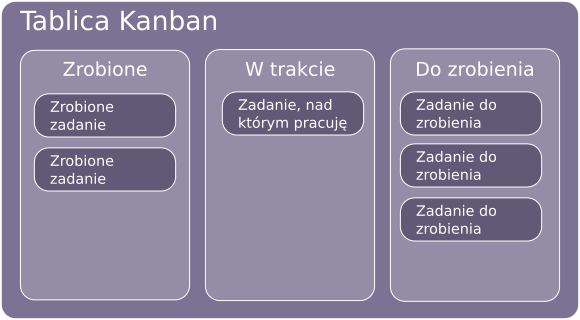
\includegraphics[width=0.90\textwidth]{tablica_kanban}		
	 \caption{Prosta tablica Kanban}
\end{figure}


Pierwotnym celem systemu Kanban było zarządzanie produkcją i redukcja jej kosztów za pomocą wizualnego sterowania. Zgodnie z systemem najpierw należy określić materiał i jego ilość potrzebną do procesu A. Informacja wraz z niezbędnymi surowcami zostaje wysłana do procesu B, tak aby produkcja mogła wystartować. Zostaje wyprodukowana konkretna ilość towaru, a po zakończeniu procesu narzędzia, pojemniki wraz z informacją  wraca do pierwotnego procesu A. Rozpoczyna  się kolejny cykl pracy. W konsekwencji produkcja jest w stanie dostosować się do zapotrzebowania klientów oraz zminimalizować ewentualną nadprodukcję, a tym samym koszty. System pozwala na koordynację pomiędzy zapotrzebowaniem a wielkością produkcji. W ten sposób narodziło się podejście Kanban, które znalazło zastosowanie poza procesami produkcyjnymi i wykorzystano je w innych dziedzinach przy zarządzaniu zadaniami.

\indent Metoda Kanban pochodzi z Japonii. Słowo kanban w języku japońskim oznacza szyld, tablicę informacyjną, kartę lub znak.  Kluczowym elementem metody jest karta Kanban. Przekazuje ona informację dotyczącą przeniesienia materiału wewnątrz zakładu lub od zewnętrznego dostawcy, w analizowanym wypadku zostaje przeniesione określenie zadanie do wykonania. Istnieje przekonanie, że systemy kierowane popytem prowadzą do mniejszej ilości zapasów oraz dynamicznych zmian w produkcji, dzięki czemu wspomagają konkurencyjność firmy. Obecnie informacje mogą być wysyłane drogą elektroniczną, co zmniejsza wykorzystanie kart. Elektroniczne podejście umożliwia eliminację błędów ręcznych czy przypadkowe zagubienie. Co ciekawe system e-kaban można zintegrować z innymi systemami, dzięki czemu otrzymujemy szersze pole danych do optymalizacji produkcji.


Opisana metoda Kanban została uproszczona i wykorzystana przy zarządzaniu małymi zespołami. Wykorzystano wizualizację procesu w formie tablicy oraz ograniczono liczbę zadań. Dzięki temu, na pierwszy rzut oka można określić nad czym się pracuje i co będzie robione w następnej kolejności. Dzięki ograniczeniu zadań, które aktualnie są wykonywane, zwiększa się wydajność zespołu. Poprzez stworzenie aplikacji i zastąpienie fizycznej tablicy, możemy dokumentować historię zadań, tworzyć statystyki, eliminować oraz śledzić błędy.


Porównując do innych metod zarządzania, metoda Kanban jest prosta w implementacji oraz jej efekty są szybciej zauważalne.  Do głównych zalet tablic Kanban należy zwiększenie wydajności i produktywności pracowników, usprawnienie komunikacji w zespole oraz doskonalenie i optymalizacja procesów. Metoda Kanban może być stosowana w różnych dziedzinach, np. sprzedaż, zarządzanie codziennymi obowiązkami lub programowanie.


\section{Aplikacja internetowa}

Aplikacja internetowa do zarządzania zadaniami jest w stanie zapewnić każdy z wypełnionych wymogów, dostarczając niezbędnych informacji na temat postępów i pozostając przyjazna dla użytkownika. Zamysł aplikacji opiera się na stworzeniu wspólnej tablicy, której celem jest przedstawić w przejrzysty sposób zadania i ich statusy. Aktualnie polecenia lub z nadanymi statusami, będą wyświetlać się jako bloki, które można przesuwać po tablicy. Jest to proste zobrazowanie postępu prac nad daną grupą zadań. Osoba zarządzająca może zobaczyć podgląd rozwoju projektu. Natomiast pracownik, który zrobił postęp w wybranym zadaniu, z łatwością jest w stanie udokumentować i wyświetlić go dla całego zespołu. 

\section{Porównanie istniejących aplikacji}
Istnieje szereg aplikacji o zbliżonej funkcjonalności. Opisane zostaną dwie aplikację: Trello i LeanKit,  ponieważ odzwierciedlają one podobieństwa i różnice pomiędzy aplikacją zaproponowaną w niniejszej pracy inżynierskiej.


Zaczynając od Trello, jest to aplikacja bazująca głównie na swej prostocie. Tablicę zadań udostępnioną za pomocą wiadomości e-mail z zaproszeniem, czy też współdzielonego hiperłącza utworzyć można zaledwie w pięć minut. Zadania na tablicy wyglądają na proste, składające się jedynie z opisu, lecz każde zadanie ma swoją stronę gdzie opis staje się bardziej zaawansowany, można dodać między innymi:
\begin{itemize}
	\item pliki, 
	\item listę podzadań,
	\item termin ostatecznego zakończenia zadania,
	\item etykiety kategoryzujące poszczególne grupy zadań,
	\item osoby wykonujące zadanie,
	\item komentarze,
\end{itemize}
Użytkownicy mogą posiadać dwie role, admina i zwykłego użytkownika. Różnią się one jedynie tym, że admin może usuwać i dodawać użytkowników oraz zmieniać ustawienia główne tablicy. Wiele funkcji takich jak przedstawianie zadań na kalendarzu, osie czasu, dodanie lokalizacji do zadań istnieją w wersji płatnej rozszerzonej. Wiele aplikacji, służących do tworzenia tablicy Kanban wzoruje się na tej aplikacji i jest ona jak dotąd jedną z najlepszych rozwiązań. Omawiana aplikacja mocno spopularyzowała metodykę zarządzania zadaniami poprzez tablicę Kanban.

\begin{figure}[h]
	\centering
	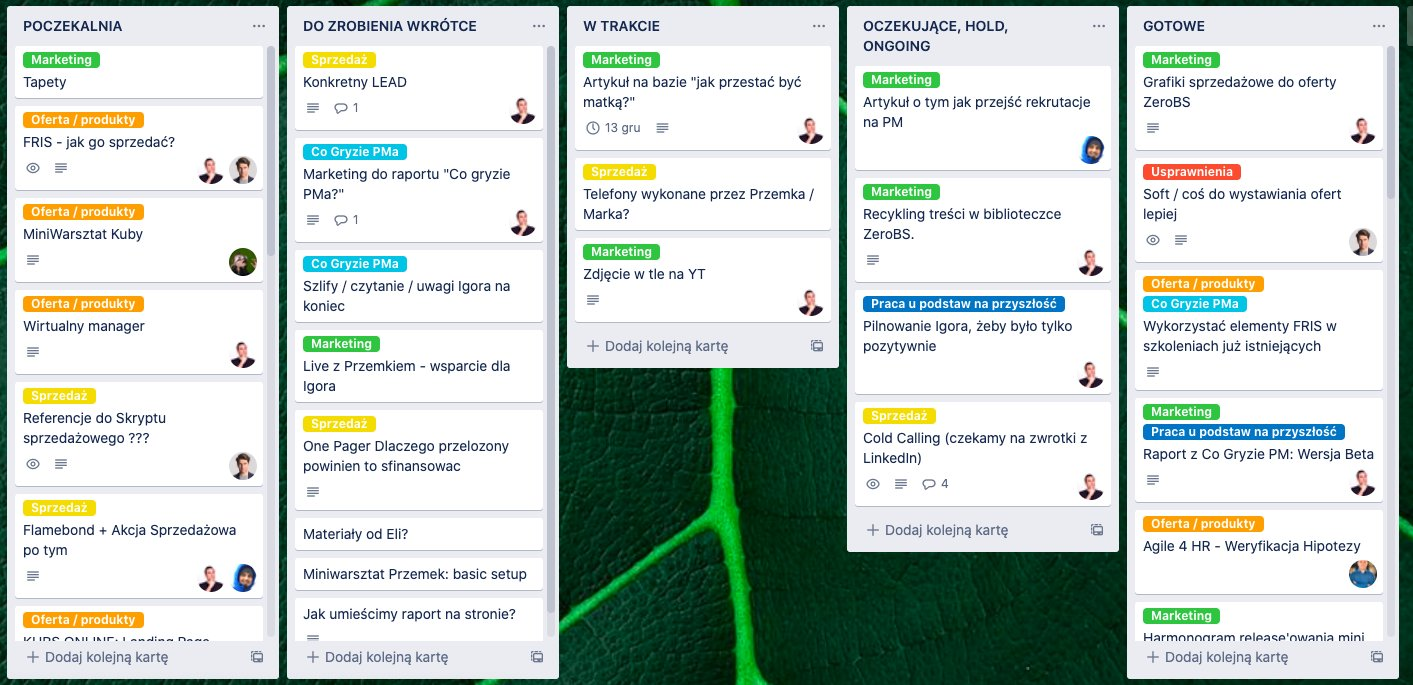
\includegraphics[width=0.90\textwidth]{tablica-operacyjna}		
	\caption{Przykładowa tablica Kanban w aplikacji Trello}
\end{figure}

\indent  Kolejną aplikacją jest LeanKit, która została wybrana jako druga aplikacja do porównania, ponieważ tej tablicy nie charakteryzuje prostota. Jej atutem są złożone funkcje tworzenia tablicy. Najbardziej charakterystyczną opcją jest skomplikowane tworzenie karty na tablicy. Poprzednia aplikacja pozwalała na tablicy utworzyć karty przetrzymujące zadania, które można przenosić z jednej karty na drugą. Aplikacja oferuje Tworzenie Karty, podkart karty, podkart podkart, i tak dalej, przez co bardziej skomplikowane do skategoryzowania zadania użytkownik jest w stanie opisać w jednym miejscu. Zadania posiadają podobne atrybuty do Trello, oprócz tego posiadają jeszcze dziedziczenie zadań, to znaczy, że każde zadanie ma listę zadań rodziców i listę zadań dzieci. Są to listy przetrzymujące odnośniki do zadań, z wyniku których powstało dane zadanie (rodzice), lub zadania, które zostały utworzone przez dane zadanie (dzieci). 
Poza skomplikowaną reprezentacją tablicy Kanban, LeanKit posiada wiele funkcji po wizualizacje zadań w kalendarzu, możliwość wertykalnej i horyzontalnej tablicy (jak i wertykalno-horyzontalnej), raporty w postach czystych danych lub wykresów czy też tworzenia zależności pomiędzy wieloma innymi projektami i tablicami.
Jest to aplikacja posiadająca kompleksowe konfiguracje, użytkownik korzystający z programu po raz pierwszy najprawdopodobniej potrzebowałby specjalistycznego szkolenia w celu wykorzystania wszystkich możliwości.


\indent Porównanie istniejących aplikacji uwydatniła cechy, które zostały wdrożone do TaskManager. Program również charakteryzuje się prostotą, lecz dopiero podczas korzystania przez zwykłego użytkownika. Proces inicjalizacji tablicy, projektów jest dłuższy, aby potem aplikacja mogła służyć uczestnikom projektu.
Pierwszą różnicą jest podział na dwie role, ADMIN, USER. Rola administratora projektu (Admin) polega na posiadaniu pełnej kontroli nad dodawaniem i konfiguracją użytkowników, zadań oraz tablic.
Drugą cechą charakterystyczną jest zakładka statystyk, gdzie zobaczyć można ogólne informacje na temat całego projektu, wyników poszczególnych użytkowników, jak i zadań w przeciągu ostatnich sześciu miesięcy.
Kluczową cechą, która może przekonać klienta do korzystania z TaskManager jest możliwość utworzenia wewnętrznego projektu niezależnego do innych aplikacji. Wraz ze wzrastającymi oczekiwaniami klient może zlecić rozszerzenie programu na swój sposób, czy to przez podłączenie do kanału komunikacyjnego lub kalendarza z grafikiem pracowniczym.





